\begin{frame}{Fundamentação Teórica}
    As seções posteriores, agruparão os conceitos em elementos: Base do projeto, \textit{Hardware}, \textit{Firmware} e \textit{Software}.  
\end{frame}

\begin{frame}{Elementos Base}{Redes \textit{Wireless}}
      
\begin{itemize}
    \item O termo \textit{Wireless} provém do inglês: \textit{wire} (fio, cabo); less (sem);
    \medskip
    \item Possui vantagens cruciais para a aplicação do conceito de Internet das Coisas:
\end{itemize}    

\end{frame}

\begin{frame}{Elementos Base}{Redes \textit{Wireless}}
      
    \begin{itemize}
        \item \textbf{Maior produtividade - } disponibiliza acesso à rede em todo o raio de alcance onde o ponto de acesso está instalado, oferecendo liberdade de deslocamento com conexão contínua;
	
        \item \textbf{Flexibilidade de instalação -} podem ser instaladas em locais com temperaturas elevadas, em que os cabos não suportariam, ou em locais que necessitam de acesso temporário;
        
        \item \textbf{Redução de custo - } reduzem os custos de instalação, dispensando o uso de material para cada ponto de conexão;
        
        \item \textbf{Interoperabilidade e segurança - } capaz de comunicar sistemas de forma confiável e com segurança, possuindo chaves de acesso e até mesmo transferindo mensagens criptografadas.   
    \end{itemize}    
    
\end{frame}

\begin{frame}{Elementos Base}{Redes \textit{Wireless}}
    A topologia de uma rede IEEE 802.11 (\textit{Wi-Fi})  possui os seguintes elementos-chave:

    \begin{itemize}
        \item \textbf{BSS - \textit{Basic Service Set} -} corresponde a uma célula de comunicação \textit{wireless};
        \item \textbf{STA - \textit{Stations} -} são as estações de trabalho que comunicam-se entre si dentro da \textbf{BSS};
        \item \textbf{AP - \textit{Access Point} -} coordena a comunicação entre as \textbf{STA's} dentro da \textbf{BSS}. Na maioria das vezes roteadores realizam tal operação;
        
    \end{itemize}
    
\end{frame}

% \begin{frame}{Elementos Base}{Redes \textit{Wireless}}
%     \begin{itemize}
%     \item \textbf{\textit{Bridge} -} faz a ligação entre diferentes redes, por exemplo, uma rede sem fio para uma rede cabeada convencional;
% 	\item  \textbf{ESS - \textit{Estended Service Set} -} consiste de várias células \textbf{BSS's} vizinhas que se interceptam e cujos \textbf{AP's} estão conectados a uma mesma rede tradicional. Nestas condições uma \textbf{STA} pode movimentar-se de um \textbf{BSS} para outra, permanecendo conectada à rede. Este processo é denominado \textit{Roaming}.
% 	\end{itemize}
% \end{frame}

\begin{frame}{Elementos Base}{A Internet das Coisas}
    \begin{itemize}
        \item Um conjunto de tecnologias e protocolos associados que permitem que objetos se conectem a uma rede de comunicações e onde são identificados e controlados;
        \item Esse termo se tornou possível graças aos avanços tecnológicos e as reduções de custo de todos os dispositivos eletroeletrônicos, os quais possuem a capacidade de comunicação principalmente por meio de protocolos \textit{Wiress};
    \end{itemize}
    
\end{frame}

\begin{frame}{Elementos Base}{A Internet das Coisas}

    \begin{figure}
        \centering
        \caption{Protocolos utilizados para aplicacão do \textit{IoT} com base nos conceitos de redes. Relação entre velocidade-força e distância.}
        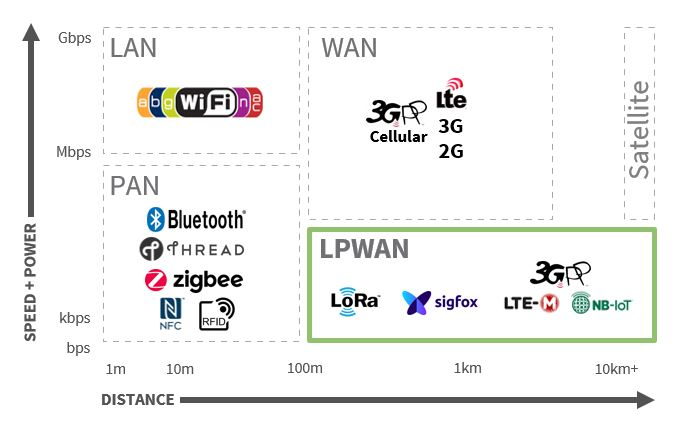
\includegraphics[width=0.6\linewidth]{figuras/iotprotocols.jpg}
        \caption*{\tiny{Fonte: iot.do, 2021}}
    \end{figure}   

\end{frame}


\begin{frame}{Elementos Base}{O protocolo MQTT}

    \begin{itemize}
        \item \textbf{\textit{Message Queuing Telemetry Transport}} - MQTT foi inventado e desenvolvido inicialmente pela \textit{International Business Machines} - IBM;
        \item É um protocolo de mensagem com suporte para a comunicação \textbf{assíncrona} entre as partes;
        \item Projetado para aplicações que utilizam pouca banda de rede utilizando um modelo de publicação e assinatura;

    \end{itemize}


\end{frame}

\begin{frame}{Elementos Base}{O protocolo MQTT}

    \begin{itemize}
        \item Em uma rede MQTT existem dois agentes principais: o \textit{\textbf{broker}} e os \textit{\textbf{clients}};
        \item O \textit{broker} é um servidor que centraliza as mensagens dos clientes e as encaminha para os clientes interessados;
        \item Um \textit{client} é um dispositivo ou serviço que tenha capacidade de interagir com o \textit{broker} e trocar mensagens;

    \end{itemize}


\end{frame}

\begin{frame}{Elementos Base}{O protocolo MQTT}

    \begin{figure}[H]
        \centering
        \caption{Diagrama básico MQTT}
        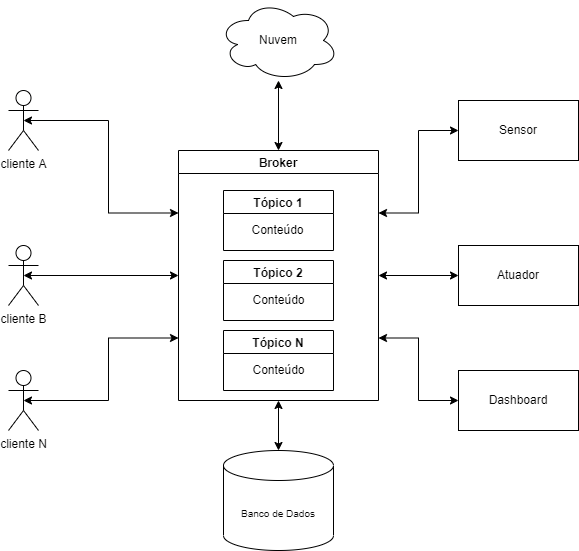
\includegraphics[width=0.45\textwidth]{figuras/mqtt.drawio.png}
        \caption*{\tiny{Fonte: própria, 2021}}
        \label{fig:mqtt_diagram}
    \end{figure}

\end{frame}

\begin{frame}{Elementos Base}{O protocolo MQTT}
    \begin{itemize}
        \item Está na mesma camada OSI que o \textbf{\textit{Hypertext Transfer Protocol}} - HTTP, porém a maior diferença entre eles é o tamanho do \textit{payload};
        \item Como qualquer outro protocolo de comunicação o MQTT possui diversos termos e características associadas, como a segurança, a definição dos \textit{endpoints}\footnote{\textbf{endpoints} - Pontos de extremidade. Terminais de conexão entre uma API e o cliente.}, o endereçamento, tipo de dado trafegado, entre outros.
    \end{itemize}

\end{frame}

\begin{frame}{Elementos Base}{O protocolo MQTT}
    \begin{itemize}
        \item \textbf{\textit{broker}}: É o intermediário no processo de comunicação, atuando como um servidor;
        \item \textbf{\textit{client}}: Responsável por estabelecer e manter uma conexão com o \textit{broker}, enviar e receber as mensagens;
        \item \textit{\textbf{broker ip}}: Identificação única do servidor \textit{\textbf{broker}} conectado em determinada rede;
        \item \textbf{\textit{broker username e broker password}}: Credenciais, opcionais, para determinado cliente estabelecer conexão com o servidor; 
    \end{itemize}

\end{frame}

\begin{frame}{Elementos Base}{O protocolo MQTT}
    \begin{itemize}
        \item  \textit{\textbf{QoS}}: Nível de qualidade do serviço desejado, indicando como deve ser a relação entre os elementos comunicantes.\cite{fabiobrandao};
        \item \textbf{\textit{last good message}}: É a operação à qual o \textit{broker} envia a última menagem válida recebida em um determinado tópico ao ser requisitado por um cliente;
        \item \textbf{\textit{last will testament (LWT)}}: São mensagens pré-definidas a serem publicadas pelo broker em nome de um determinado cliente, uma vez que esse cliente está \textit{offline} e não pode publicar mais;
        \item \textbf{\textit{keep alive}}: Mensagens periódicas enviadas por determinado cliente buscando validar a conexão;
    \end{itemize}

\end{frame}

\begin{frame}{Elementos Base}{O protocolo MQTT}
    \begin{itemize}
        \item \textbf{tópicos, \textit{publish} e \textit{subscribe}}: O ato de um cliente enviar uma mensagem é chamado \textit{publish}(publicação). E para receber mensagens de determinado um tópico um cliente deve fazer um \textit{subscribe}(inscrição). Os níveis de um tópico são separados por “/” e um cliente pode optar por se inscrever em quantos tópicos forem necessários, utilizando os artifícios da \autoref{tab:simbolos_mqtt}.
    \end{itemize}

\end{frame}

\begin{frame}{Elementos Base}{O protocolo MQTT}
    \begin{table}[H]
        \centering
        \resizebox{\textwidth}{!}{%
            \begin{tabular}{c|c|c}
                \hline
                Símbolos & Descrição & Exemplo \\ \hline
                + & Retorna ou envia qualquer informação naquele nível (Coringa) & \begin{tabular}[c]{@{}c@{}}area/10/sensor/5000/temperatura\\ area/10/sensor/4000/temperatura\\ area/10/sensor/+/temperatura\end{tabular} \\ \hline
                \# & Retorna ou envia qualquer coisa abaixo daquele nível & area/10/\# \\ \hline
                \$ & Tópicos iniciados com \$ são especiais usados internamente pelo broker. & \$SYS/broker/clients/total \\ \hline
            \end{tabular}%
        }
        \caption{Caracteres especiais utilizados para envio e recebimento no protocolo MQTT.}
        \label{tab:simbolos_mqtt}
    \end{table}

\end{frame}


\begin{frame}{Elementos de \textit{Hardware}}{O microcontrolador ESP8266}
    \begin{itemize}
        \item É um \textit{chip} microcontrolador da fabricante chinesa \textit{Espressif Systems} construído em torno de um processador Tensilica Xtensa LX3, inclui \textit{Wi-Fi on-board}.
    \end{itemize}

    \begin{figure}[H]
        \centering
        \caption{\textit{ESP8266EX}.}
        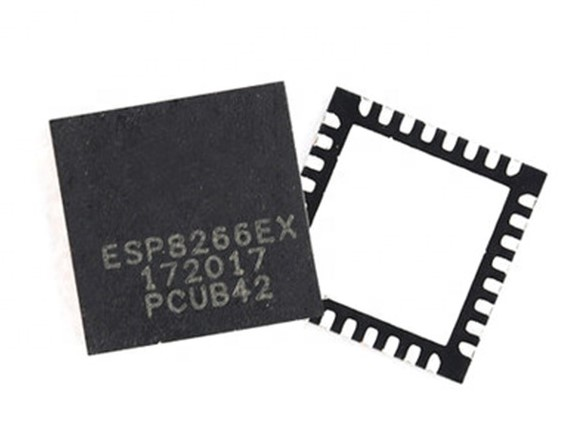
\includegraphics[width=0.3\textwidth]{figuras/esp8266ex.jpg}
        \caption*{\tiny{Fonte: digikey.com, 2021}}
        \label{fig:esp8266ex}
    \end{figure} 
\end{frame}

\begin{frame}{Elementos de \textit{Hardware}}{O microcontrolador ESP8266}
    \begin{itemize}
        \item Rapidamente se tornou popular como um microcontrolador autônomo devido ao seu baixo custo de mercado;
        \item Integração com a plataforma \textit{Arduino};
        \item Criação de \textit{kits} de desenvolvimento.
    \end{itemize}

\end{frame}

\begin{frame}{Elementos de \textit{Hardware}}{O microcontrolador ESP8266}
    \vspace*{-0.4cm}
    \begin{figure}[!ht]
        \centering
        \hspace*{0.1cm}
        \begin{minipage}{0.5\linewidth}
            \centering
            \caption{ESP-12S}
            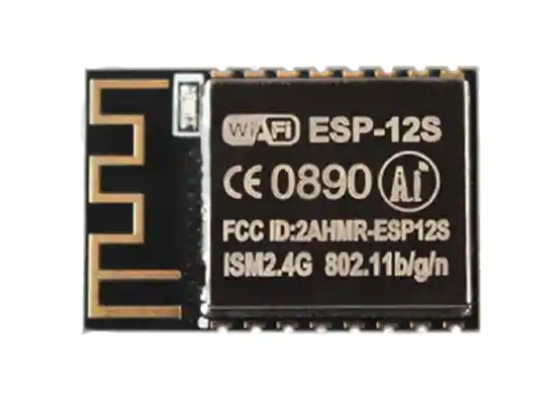
\includegraphics[width=0.4\textwidth]{figuras/ESP-12S.png}
            \label{fig:esp12s}
            \caption*{\tiny{Fonte: filipeflop.com, 2020}}
        \end{minipage}\hfill
        \begin{minipage}{0.5\linewidth}
            \centering
            \caption{ESP-12E}
            \hspace*{0.5cm}
            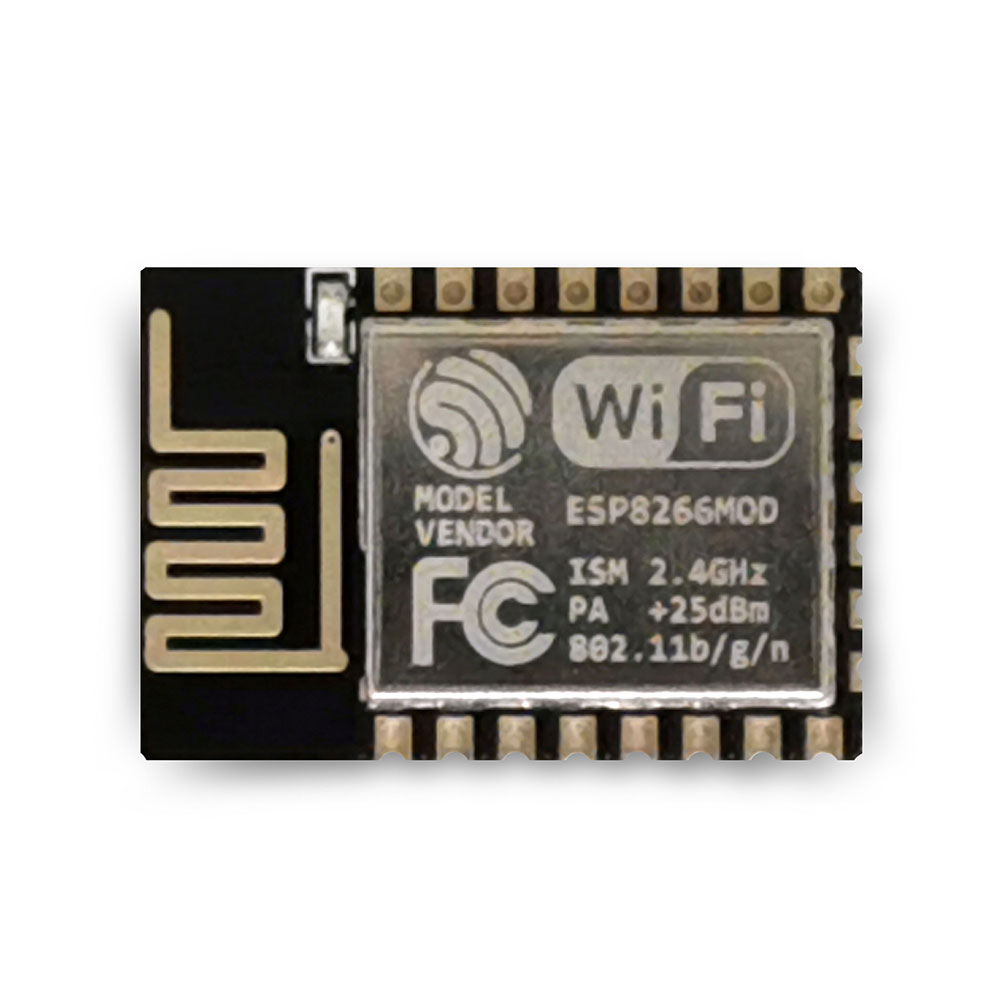
\includegraphics[width=0.4\textwidth]{figuras/ESP-12E.png}
            \label{fig:esp12e}
            \vspace*{-0.5cm}
            \caption*{\tiny{Fonte: filipeflop.com, 2020}}
        \end{minipage}
    \end{figure}

\end{frame}

\begin{frame}{Elementos de \textit{Hardware}}{O microcontrolador ESP8266}
    \vspace*{-0.4cm}
    \begin{figure}[!ht]
        \centering
        \hspace*{0.1cm}
        \begin{minipage}{0.5\linewidth}
            \centering
            \caption{Wemos D1 com ESP12-S}
            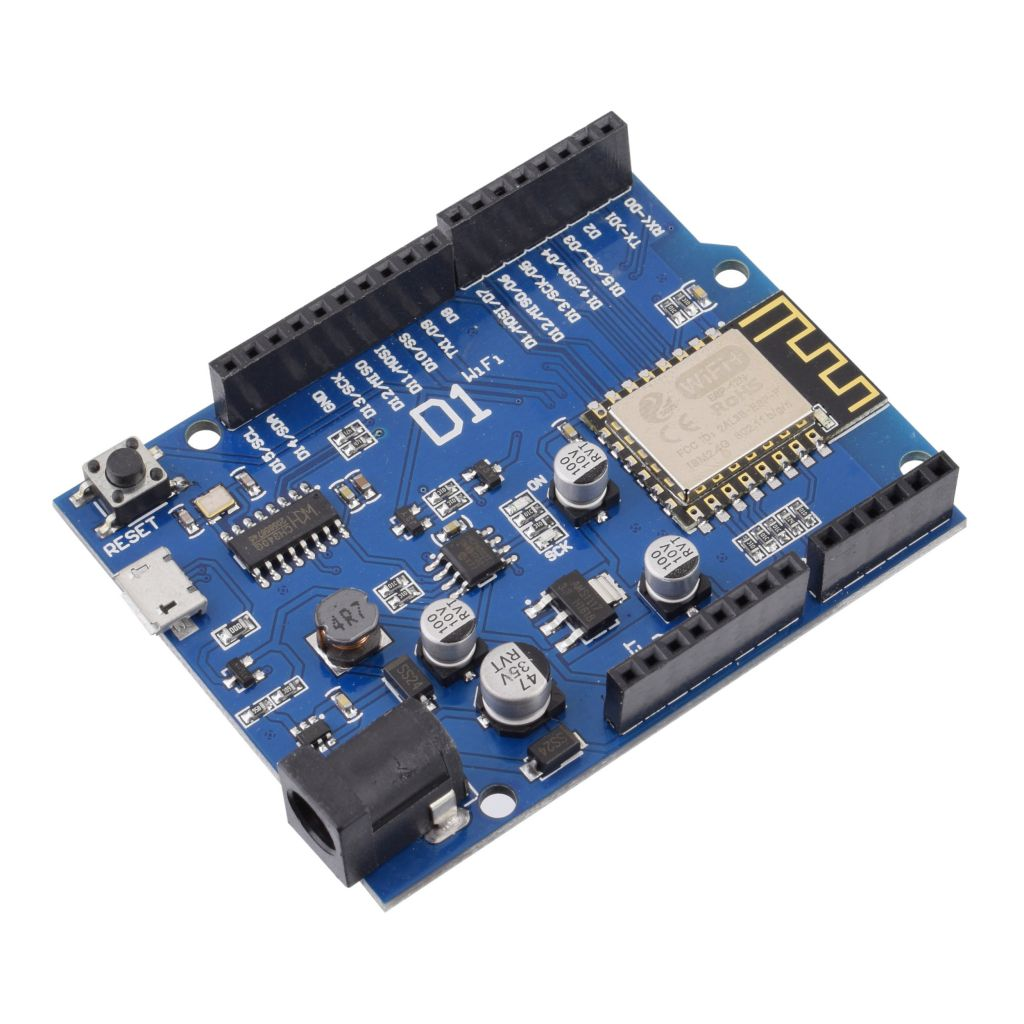
\includegraphics[width=0.4\textwidth]{figuras/ESP-12S-wemos.png}
            \label{fig:wemosesp12s}
            \caption*{\tiny{Fonte: filipeflop.com, 2020}}
        \end{minipage}\hfill
        \begin{minipage}{0.5\linewidth}
            \centering
            \caption{Nodemcu com ESP12-E}
            \hspace*{0.5cm}
            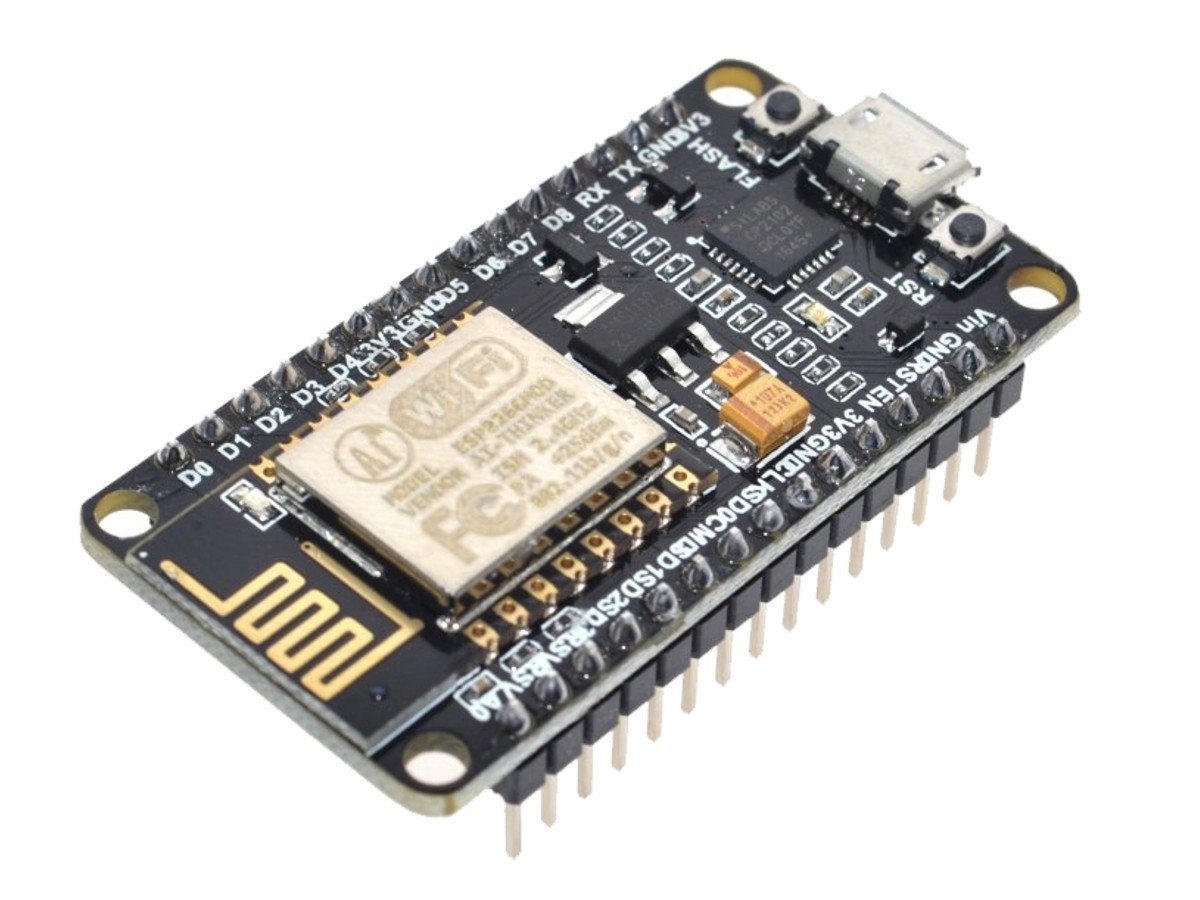
\includegraphics[width=0.4\textwidth]{figuras/ESP-12E-nodemcu.png}
            \label{fig:nodemcuesp12e}
            \vspace*{-0.5cm}
            \caption*{\tiny{Fonte: filipeflop.com, 2020}}
        \end{minipage}
    \end{figure}

\end{frame}

\begin{frame}{Elementos de \textit{Hardware}}{A Raspberry Pi Zero W}
    \begin{figure}[H]
        \centering
        \caption{Vista superior da \textit{Raspberry Pi Zero W}}
        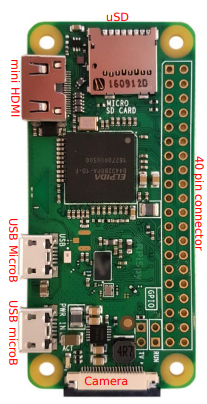
\includegraphics[width=0.2\textwidth, angle = 90]{figuras/rasp_zerow.png}
        \caption*{\tiny{sparkfun, 2020}}
        \label{fig:rasppizerow}
    \end{figure} 

\end{frame}

\begin{frame}{Elementos de \textit{Hardware}}{A Raspberry Pi Zero W}
    \begin{itemize}
        \item Compacta, ficando no meio termo entre as fazes de prototipação e aplicação;
        \item Possui conectividade \textit{Wi-Fi} e \textit{Bluetooth};
        \item Microprocessador \textit{ARM BCM2835} de \textit{1GHz}, memória \textit{RAM} de \textit{512MB};
        \item Ideal para rodar aplicações como um \textit{Broker MQTT};
    \end{itemize}

\end{frame}

\begin{frame}{Elementos de \textit{Hardware}}{As fontes de alimentação DC}
    \begin{itemize}
        \item Dois tipos de fontes chaveadas: de \textit{12V/20A} para o módulo \textbf{CCM} e \textit{12V/10A} para o módulo \textbf{TCM}.
    \end{itemize}

    \begin{figure}[H]
        \centering
        \caption{Vista superior da fonte}
        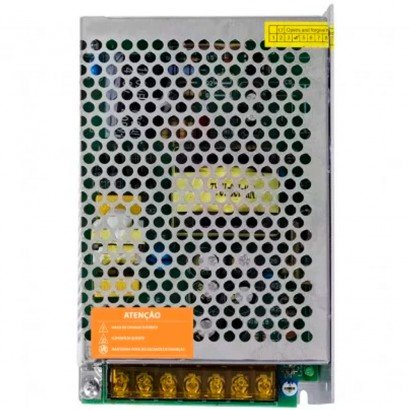
\includegraphics[width=0.2\textwidth]{figuras/fonte_chaveada.jpg}
        \caption*{\tiny{amazon, 2020}}
        \label{fig:fontechaveada}
    \end{figure} 

\end{frame}


\begin{frame}{Elementos de \textit{Hardware}}{A motobomba}
    \begin{itemize}
        \item Trabalha com fontes de alimentação de correntes contínuas (\textit{DC});
        \item Opera a \textit{12V}, com potência máxima de \textit{80W};
        \item Capacidade de exercer uma vazão de \textit{5,5L/min} com ganho de elevação de no máximo 40\textit{m}.
    \end{itemize}

    \begin{figure}[H]
        \centering
        \caption{Bomba d'água \textit{DC}}
        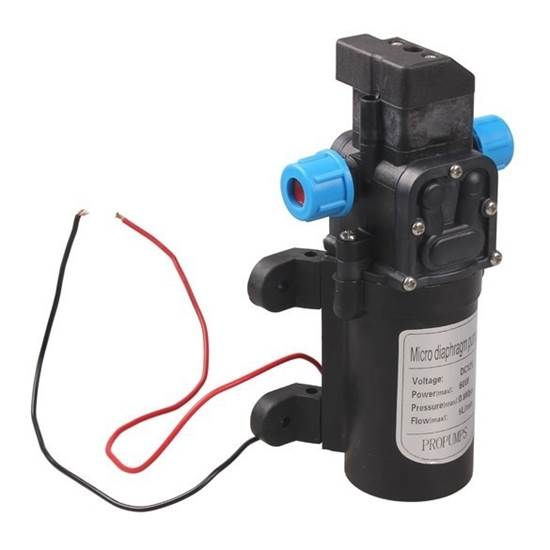
\includegraphics[width=0.2\textwidth]{figuras/bomba.jpeg}
        \caption*{\tiny{ENERGIA TOTAL, 2020}}
        \label{fig:bomba}
    \end{figure}

\end{frame}

\begin{frame}{Elementos de \textit{Hardware}}{O sensor ultrassônico}
    \begin{itemize}
        \item {É um instrumento que mede a distância até um objeto usando ondas sonoras de frequência acima do alcance da audição humana;}
        \item {Usa um transdutor para enviar e receber pulsos ultrassônicos os quais são utilizados para medição de distância através de lapsos temporais;}
    \end{itemize}
\end{frame}

\begin{frame}{Elementos de \textit{Hardware}}{O sensor ultrassônico}
    \begin{equation}
        d = \frac{\Delta t \cdot v}{2}
        \end{equation}
        \\
        \begin{itemize}
            
            \item $d$ é a distância;
            \item $\Delta t$ é a diferença entre o tempo de emissão e chegada da onda;
            \item  $v$ é a velocidade do som (tomada como $340m/s$). \\
        \end{itemize}

        \begin{figure}[H]
            \centering
            \caption{Representação do funcionamento de um sensor ultrassônico}
            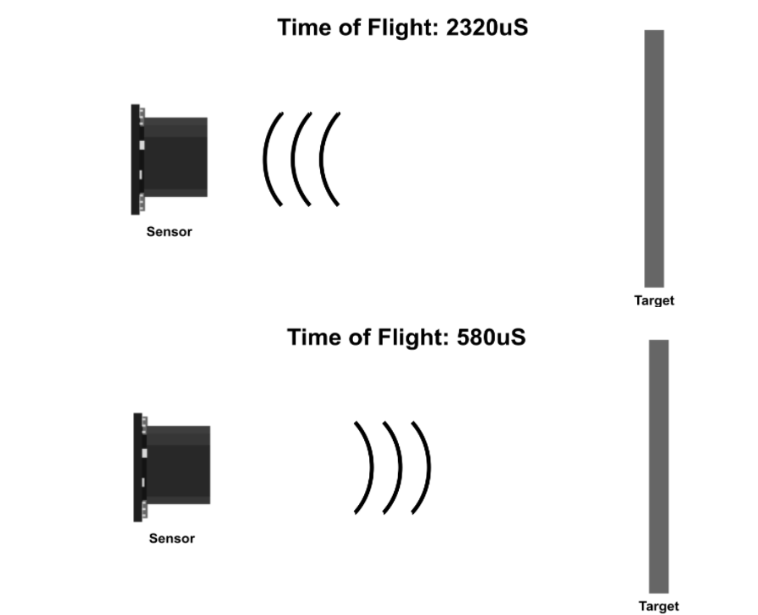
\includegraphics[width=0.3\textwidth]{figuras/ultrassonico_operacao.png}
            \caption*{\tiny{Maxbotix, 2021}}
            \label{fig:operacao_ultrassonico}
        \end{figure}
        
\end{frame}

\begin{frame}{Elementos de \textit{Hardware}}{O sensor ultrassônico}
  
\begin{figure}[H]
	\centering
	\caption{Sensor ultrassônico JSN-SR04T.}
	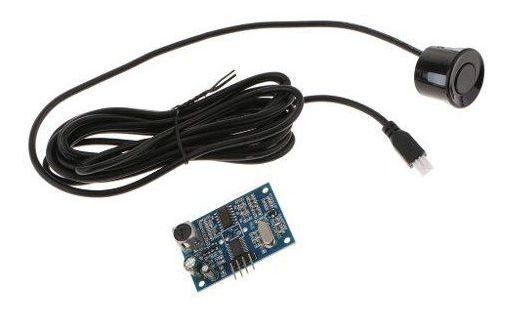
\includegraphics[width=0.4\textwidth]{figuras/sensor_ultra.jpg}
	\caption*{\tiny{usinainfo.com}, 2020}
	\label{fig:sensor_ultra}
\end{figure}
        
\end{frame}

\begin{frame}{Elementos de \textit{Hardware}}{O sensor ultrassônico}
  \begin{itemize}
      \item Módulo de apenas quatro pinos: \textit{5V} (VCC), \textit{Trig (RX)}, \textit{Echo (TX)} e \textit{GND};
      \item Possui três modos de operação sendo selecionados pelo valor do resistor (R27);
      \item \textbf{Modo de operação 3 (R27 $= 120k\Omega$)}: neste modo, o microcontrolador entra em modo de baixo consumo e só envia os dados de leituras ao ser acionado pelo pino RX. Se a mensagem de acionamento for 0X55, a leitura de distância é enviada pelo TX da mesma forma do modo anterior.
  \end{itemize}    

\end{frame}

\begin{frame}{Elementos de \textit{Hardware}}{A válvula solenoide}
    \begin{figure}[H]
        \centering
        \caption{Válvula solenoide}
        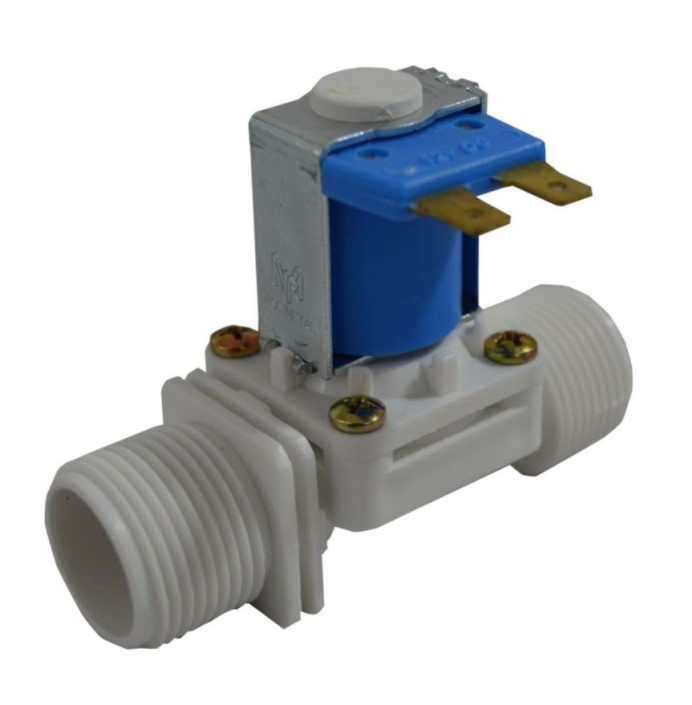
\includegraphics[width=0.2\textwidth]{figuras/solenoide.jpg}
        \caption*{\tiny{Nascimetal, 2021}}
        \label{fig:solenoide}
    \end{figure}

    \begin{itemize}
        \item Tensão de operação em torno de \textit{12V} \textit{DC}, consumo médio, quando ativada, de \textit{500mA};
        \item Pressão de operação à $8,0 kgf/cm^2$ com vazão máxima de $40L/min$ e vida útil de 50 mil operações.
    \end{itemize}    
  
\end{frame}

\begin{frame}{Elementos de \textit{Hardware}}{A chave de nível tipo boia}
    \begin{figure}[H]
        \centering
        \caption{Chave de nível \textit{RF-0H21D}}
        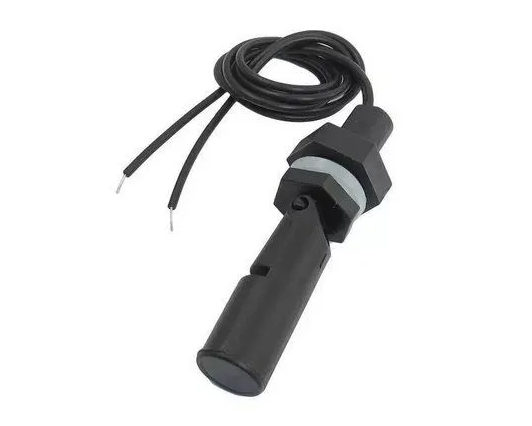
\includegraphics[width=0.3\textwidth]{figuras/chave_boia.png}
        \caption*{\tiny{smartkits, 2020}}
        \label{fig:chaveboia}
    \end{figure}

    \begin{itemize}
        \item Utilizada para fomentar a redundância do sistema, caso aconteçam falhas na medição do sensor ultrassônico.
    \end{itemize}    
  
\end{frame}

\begin{frame}{Elementos de \textit{Hardware}}{O sensor de corrente}
    \begin{figure}[H]
        \centering
        \caption{Representação gráfica do sensor \textit{ACS712}}
        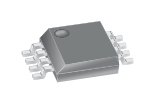
\includegraphics[width=0.15\textwidth]{figuras/ACS712.png}
        \caption*{\tiny{Alegro, 2020}}
        \label{fig:acs712}
    \end{figure}

    \begin{figure}[H]
        \centering
        \caption{Aplicação típica do\textit{ACS712}}
        \hspace*{0.1cm}
        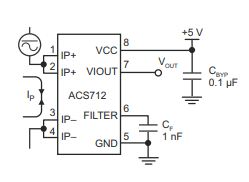
\includegraphics[width=0.25\textwidth]{figuras/ACS712_typical.png}
        \caption*{\tiny{Alegro, 2020}}
        \label{fig:acs712_typical}
    \end{figure}

\end{frame}

\begin{frame}{}
    \begin{equation}
        V_H = R_H\left ( \frac{I\cdot B}{t} \right)
        \end{equation}
        
        \begin{itemize}
            
            \item $V_H$ é a tensão em Volts;
            \item $R_H$ é o coeficiente do efeito \textit{Hall};
            \item  $I$ é o fluxo de corrente em Amperes;
            \item $t$ é espessura do sensor em milímetros;
            \item $B$ é a densidade do fluxo magnético em teslas; \ \\
        \end{itemize}

        \begin{figure}[H]
            \centering
            \caption{Comportamento da tensão de saída em relacão ao fluxo magnético de um sensor \textit{Hall}.}
            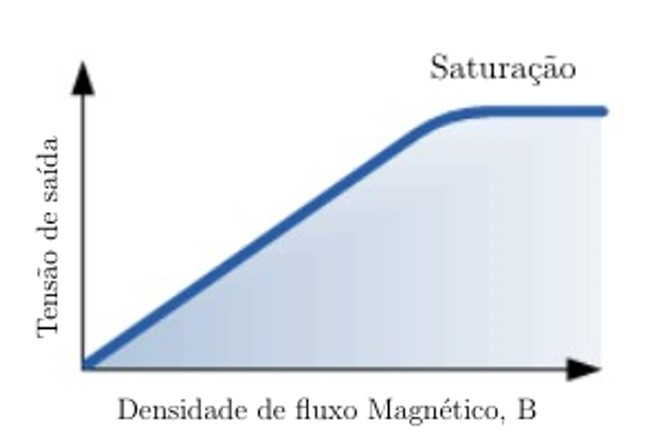
\includegraphics[width=0.3\textwidth]{figuras/grafico_hall.jpg}
            \caption*{\tiny{Eletronics Tutorials, 2021}}
            \label{fig:efeito_hall}
        \end{figure} 

\end{frame}

\begin{frame}{Elementos de \textit{Hardware}}{Kicad}
    \begin{figure}[H]
        \centering
        \caption{Exemplo de \textit{PCB Design} utilizando \textit{Kicad}}
        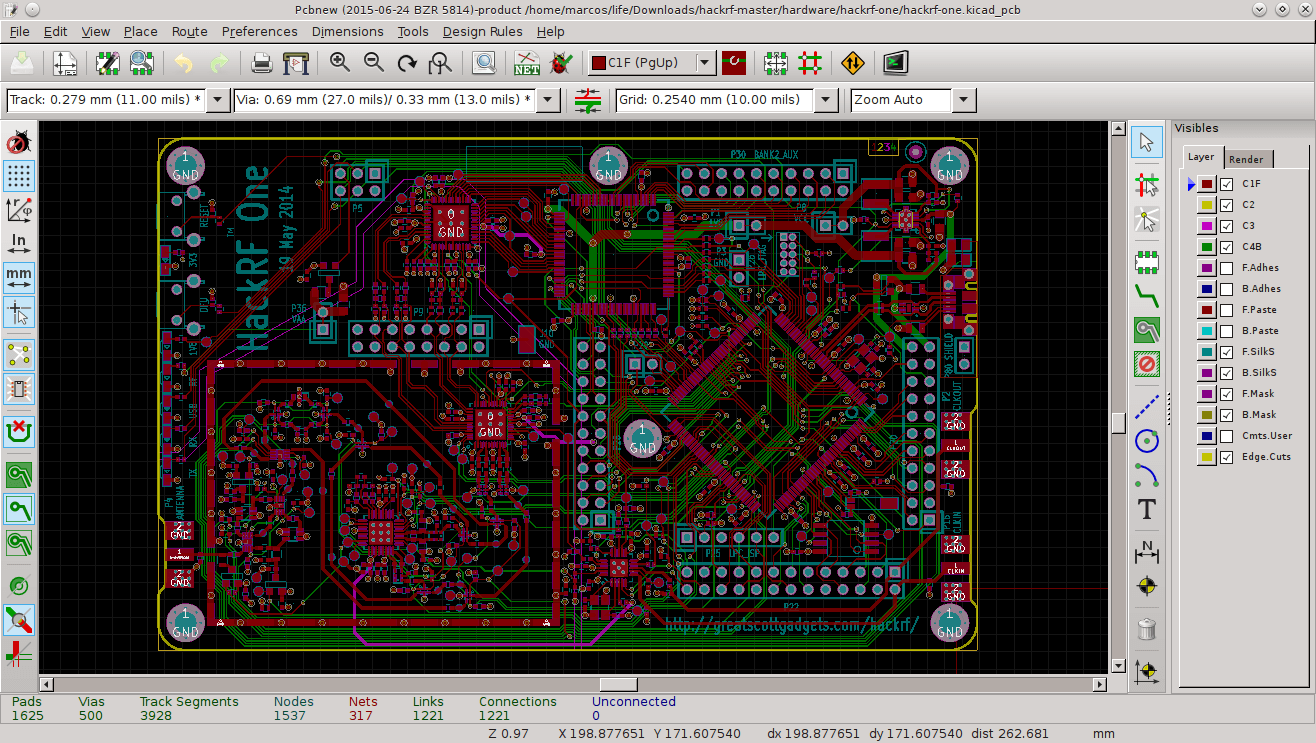
\includegraphics[width=0.5\textwidth]{figuras/kicad_pcbnew.png}
        \caption*{\tiny{kicad.org, 2021}}
        \label{fig:kicad_pcbnew}
    \end{figure} 

\end{frame}


\begin{frame}{Elementos de \textit{Firmware}}{PlatformIO}


\begin{figure}[H]
	\centering
	\caption{Extensão do \textit{PlatformIO} rodando no \textit{Visual Studio Code}}
	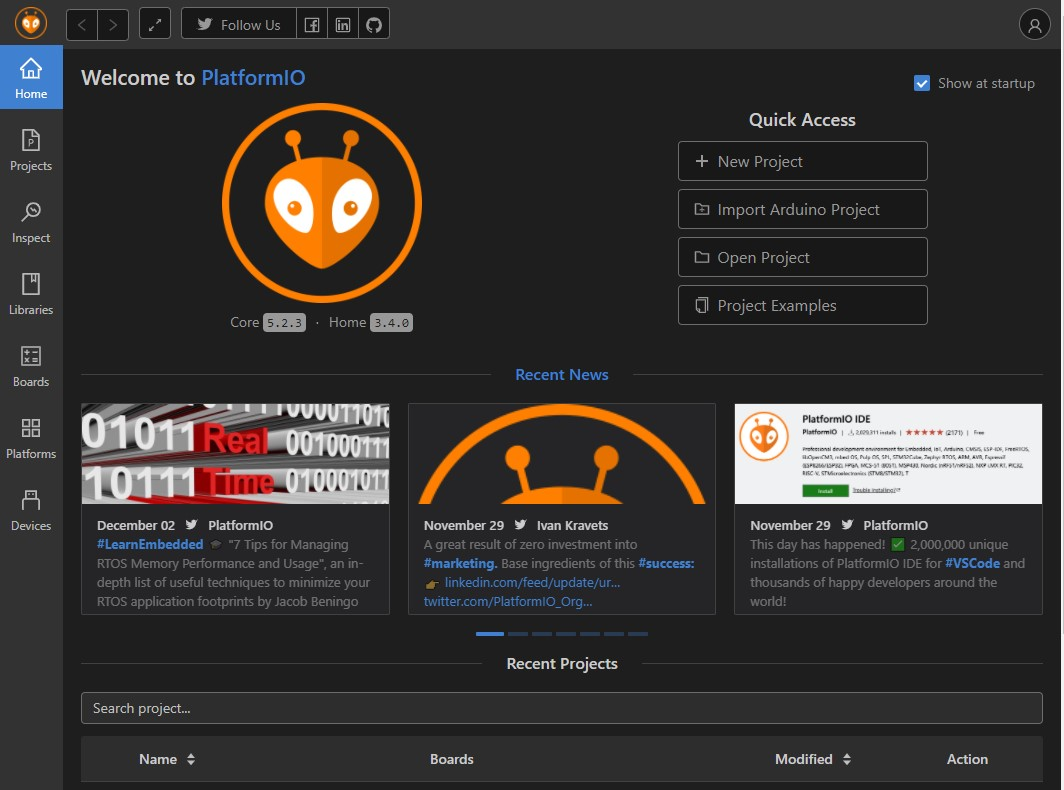
\includegraphics[width=0.5\textwidth]{figuras/platformio.jpg}
	\caption*{\tiny{Própria, 2021}}
	\label{fig:platformio}
\end{figure}
\end{frame}

\begin{frame}{Elementos de \textit{Firmware}}{A distribuição DietPi}
    \begin{figure}[H]
        \centering
        \caption{Catálogo com algumas de placas que suportam a distribuição DietPi.}
        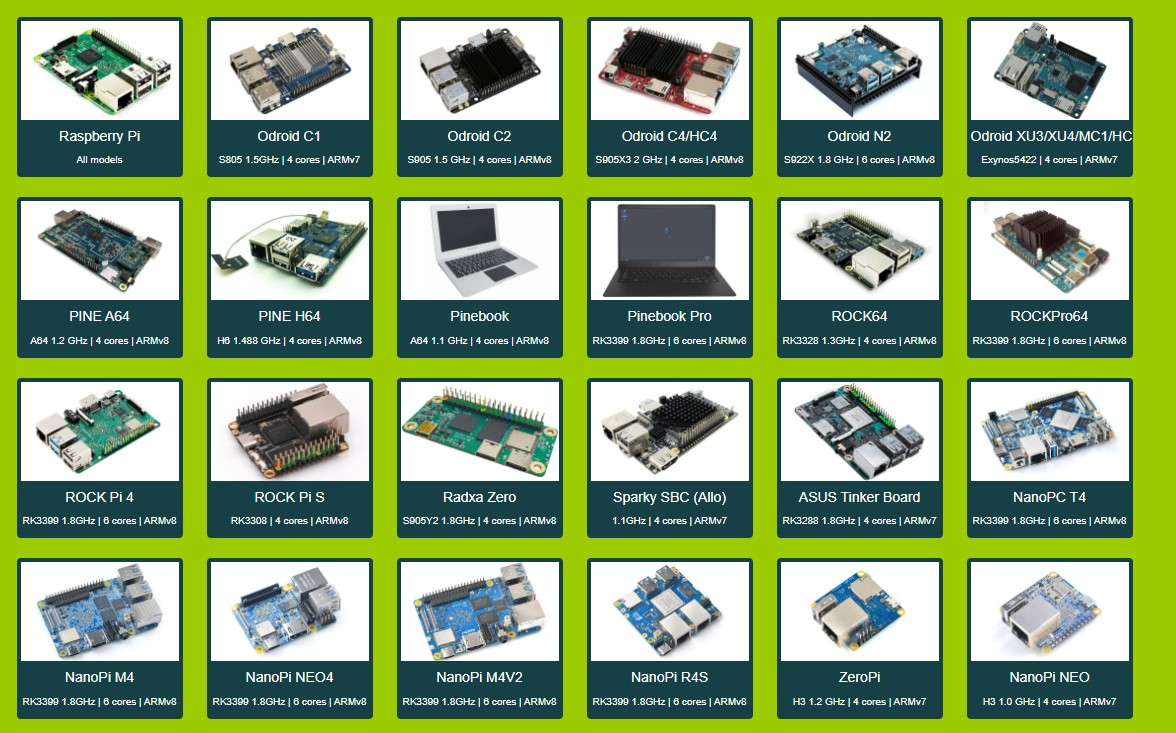
\includegraphics[width=0.5\textwidth]{figuras/dietpi.jpg}
        \caption*{\tiny{dietpi.com, 2021}}
        \label{fig:dietpi}
    \end{figure} 
\end{frame}

\begin{frame}{Elementos de \textit{Software}}{Node.js}

    \begin{itemize}
        \item É um ambiente de execução (\textit{runtime}) \textit{Javascript} possibilitando criar aplicações sem depender de um \textit{browser} para a execução;
        \item Possível empregar o \textit{Javascript} para executar comandos em terminal assim como utilizá-lo para programar qualquer tipo de aplicação \textit{backend} com auxílio de inúmeras bibliotecas desenvolvidas;
    \end{itemize}

\end{frame}


\begin{frame}{Elementos de \textit{Software}}{Electron.js}

    \begin{figure}[H]
        \centering
        \caption{Aplicações que utilizam \textit{Electron}}
        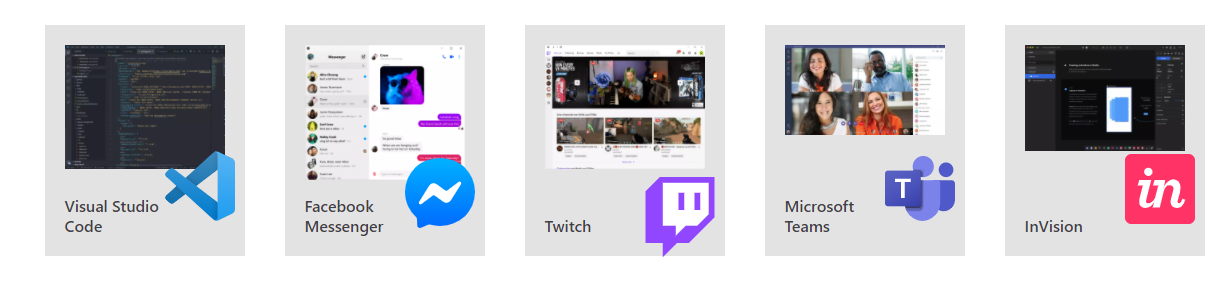
\includegraphics[width=1.0\textwidth]{figuras/electron_apps.png}
        \caption*{\tiny{Adaptado (electronjs.org, 2020)}}
        \label{fig:electron_apps}
    \end{figure}

\end{frame}

\begin{frame}{Elementos de \textit{Software}}{Electron.js}
    Uma aplicação \textit{Electron} tem como base os seguintes arquivos:

\begin{itemize}
	\item \textbf{\textit{package.json}}: Aponta para o arquivo principal do aplicativo e lista seus detalhes e dependências;
	\item \textbf{\textit{main.js}}: Inicia a aplicação e cria a janela de visualização possibilitando diversas configurações; 
	\item \textbf{\textit{index.html}}: O ponto de partida para a renderização.
\end{itemize}

\end{frame}

\begin{frame}{Elementos de \textit{Software}}{React}

    \begin{figure}[H]
        \centering
        \caption{Exemplo de componente \textit{React}}
        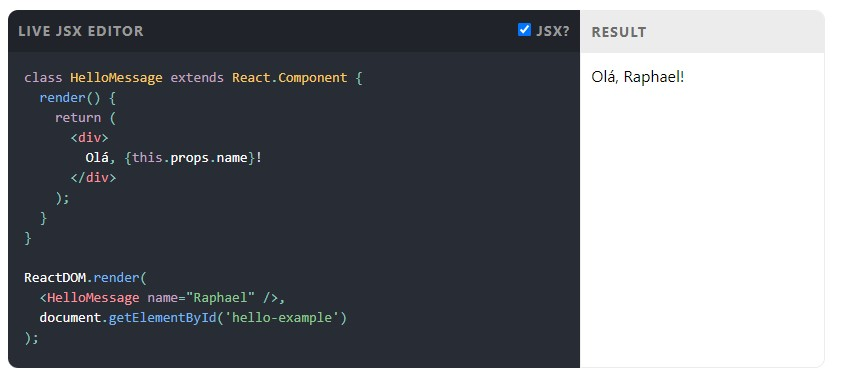
\includegraphics[width=0.8\textwidth]{figuras/exemplo_react.jpg}
        \caption*{\tiny{Adaptado (reactjs.org, 2021)}}
        \label{fig:react_code}
    \end{figure}

\end{frame}

\begin{frame}{Elementos de \textit{Software}}{React Native}
    \begin{itemize}
        \item É um \textit{framework} de codigo aberto desenvolvido pela equipe do \textit{Facebook} que suporta a criação de aplicativos \textit{mobile} multiplataforma (\textit{Android} e \textit{iOS}), sem que haja a preocupação de lidar com as linguagens padrões como \textit{Java} ou \textit{Swift}, usando apenas \textit{Javascript};
    \end{itemize}

    \begin{figure}[H]
        \centering
        \caption{Exemplos de \textit{Templates} produzidos com \textit{React Native}}
        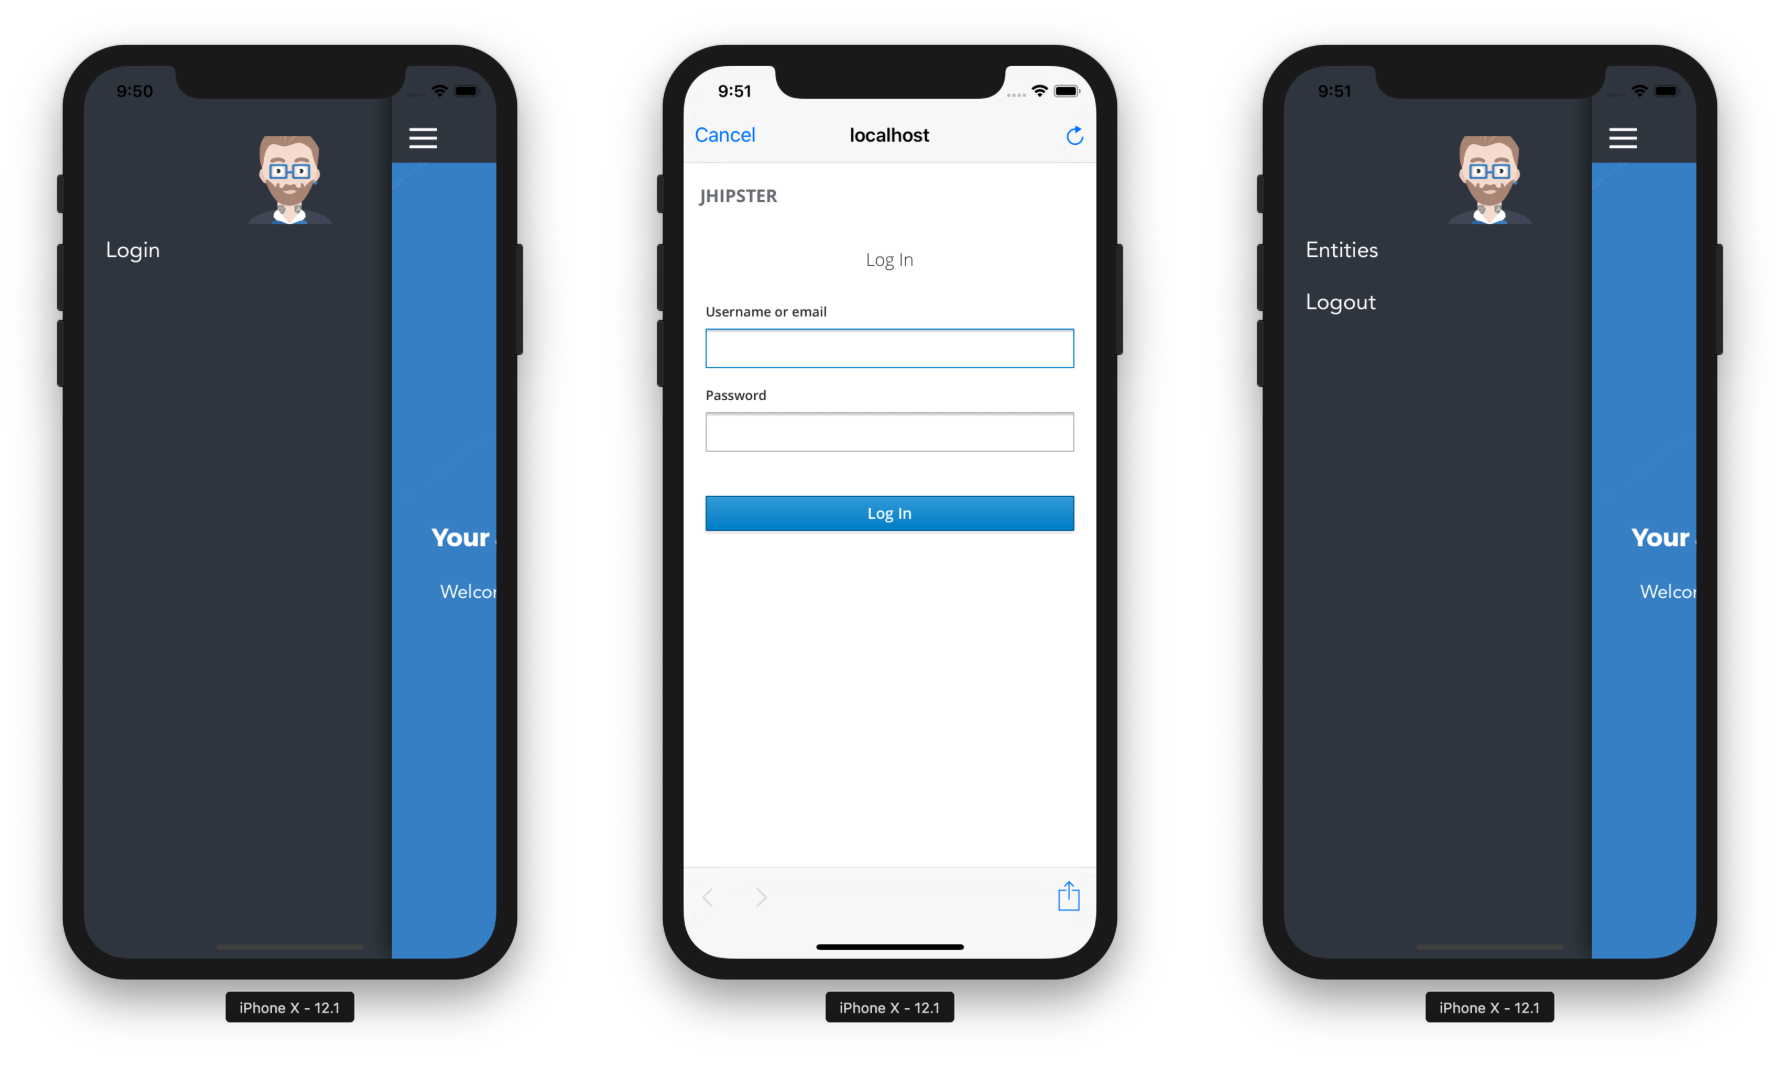
\includegraphics[width=0.5\textwidth]{figuras/react_native_elements.png}
        \caption*{\tiny{Adaptado (developer.oka, 2021)}}
        \label{fig:react-native}
    \end{figure} 

\end{frame}